\documentclass[11pt,a4paper]{scrartcl}
\usepackage{typearea}
\usepackage{mathptmx}
\usepackage[T1]{fontenc}
\DeclareMathAlphabet{\mathcal}{OMS}{cmsy}{m}{n}
\usepackage[super]{nth}
\usepackage{graphicx} % Required for inserting images
\usepackage{amsmath}
\usepackage{amsthm}
\usepackage{amsfonts}
\usepackage{amssymb}
\usepackage{physics}
\usepackage[shortlabels]{enumitem}  
\DeclareSymbolFont{sfoperators}{OT1}{cmss}{m}{n}
\DeclareSymbolFontAlphabet{\mathsf}{sfoperators}

\usepackage{tikz}
\usetikzlibrary{fit,shapes,calc,matrix,math,positioning,arrows.meta,fpu,patterns,patterns.meta,fadings}

%https://tex.stackexchange.com/questions/22801/correct-delimiter-height-in-tikz
%see solution by Martin Scharrer
\makeatletter
\def\tikz@delimiter#1#2#3#4#5#6#7#8{%
  \bgroup
    \pgfextra{\let\tikz@save@last@fig@name=\tikz@last@fig@name}%
    node[outer sep=0pt,inner sep=0pt,draw=none,fill=none,anchor=#1,at=(\tikz@last@fig@name.#2),#3]
    {%
      {\nullfont\pgf@process{\pgfpointdiff{\pgfpointanchor{\tikz@last@fig@name}{#4}}{\pgfpointanchor{\tikz@last@fig@name}{#5}}}}%
      \delimitershortfall\z@% as suggested by morbusg (maximum space not covered by a delimiter = 0)
      \resizebox*{!}{#8}{$\left#6\vcenter{\hrule height .5#8 depth .5#8 width0pt}\right#7$}%
    }
    \pgfextra{\global\let\tikz@last@fig@name=\tikz@save@last@fig@name}%
  \egroup%
}
\makeatother

\makeatletter
\def\operator@font{\mathgroup\symsfoperators}
\makeatother

\newcommand{\apo}{%
  \mathrel{%
    \tikz[baseline=(current bounding box.center),scale=.3]{
    \def\x{1}
    \def\y{2}
    \def\r{1.5}
    \draw (0,0) -- (\x,0);
    \draw (0,0) -- (\r*\x,\y);
    \draw (.5*\x,0) -- (\r*\x,\y);
    \draw (\x,0) -- (\r*\x,\y);
    }
  }%
}%

\newcommand{\lcone}{%
  \mathrel{%
    \tikz[baseline=(current bounding box.center),scale=.3]{
    \coordinate (a) at (-1,-1);
    \coordinate (b) at (1,-1);
    \coordinate (c) at (1,1);
    \coordinate (d) at (-1,1);
    \draw (a) -- (c);
    \draw (b) -- (d);
    \draw[dash pattern=on 2pt off 1pt] (b) arc [start angle=0, end angle=180, x radius=1, y radius=0.25];
    \draw (a) arc [start angle=180, end angle=360, x radius=1, y radius=0.25];
    \draw (c) arc [start angle=0, end angle=360, x radius=1, y radius=0.25];
    }
  }%
}%
\DeclareMathOperator{\range}{range}
\DeclareMathOperator{\domain}{domain}
\DeclareMathOperator{\nspace}{null}
\DeclareMathOperator{\Span}{Span}
\newcommand{\lmap}[2]{\mathcal{L}(#1,#2)}
\newcommand{\RR}{\mathbb{R}}
\newcommand{\FF}{\mathbb{F}}
%\newtheoremstyle{solve}% name of the style to be used
%  {10pt}% measure of space to leave above the theorem. E.g.: 3pt
%  {10pt}% measure of space to leave below the theorem. E.g.: 3pt
%  {}% name of font to use in the body of the theorem
%  {}% measure of space to indent
%  {\bfseries}% name of head font
%  {:}% punctuation between head and body
%  {5pt}% space after theorem head; " " = normal interword space
%  {}

%\theoremstyle{solve}
%\newtheorem{problem}{Problem}
%\newtheorem*{solution}{Solution}
\newcounter{problem}
\NewDocumentEnvironment{problem}{o m +m}
{ % beginning code
    \refstepcounter{problem}
    \IfNoValueTF{#1}
    { % optional is empty
        \par\medskip\noindent \textbf{Problem \theproblem}: #2
        \vspace{-1ex}\newline\rule{\textwidth}{0.5pt}
        \newline\textbf{Solution:} #3
        \vspace{-1ex}\newline\rule{\textwidth}{0.5pt}
    }
    { % optional has value
        \par\medskip\noindent \textbf{Problem \theproblem} (#1): #2
        \vspace{-1ex}\newline\rule{\textwidth}{0.5pt}
        \newline\textbf{Solution:} {#3}
        \vspace{-1ex}\newline\rule{\textwidth}{0.5pt}
    }
}
{ % end code
    \medskip
}

\NewDocumentCommand\tikzproblem{o +m +m}
{ 
    \refstepcounter{problem}
    \IfNoValueTF{#1}
    { % optional is empty
        \begin{center}
            \begin{tikzpicture}
                \node[rectangle,draw,inner sep=5pt,text width=.95\textwidth,] (problem) at (0,0) 
                {\textbf{Problem \theproblem}: #2};  
                \node[draw,rectangle,scale=.4,fill=white,opacity=1] at (problem.north west) {$\apo$};
                \node[draw,rectangle,scale=.4,fill=white,opacity=1] at (problem.north east) {$\apo$};
                \node[draw,rectangle,scale=.4,fill=white,opacity=1] at (problem.south east) {$\apo$};
                \node[draw,rectangle,scale=.4,fill=white,opacity=1] at (problem.south west) {$\apo$};
%                \node[rectangle,draw,inner sep=5pt,text width=.95\textwidth,] (solution) [below=of problem]
%                {\textbf{Solution:} #3};
            \end{tikzpicture}
        \end{center}
        \noindent
        \begin{tikzpicture}
            \draw[line cap=rect] (0,0) -- (\linewidth-\pgflinewidth,0);
        \end{tikzpicture}
        \textbf{Solution:} #3
        \\ \noindent
        \begin{tikzpicture}
            \draw[line cap=rect] (0,0) -- (\linewidth-\pgflinewidth,0);
        \end{tikzpicture}
    }
    {
        \begin{center}
            \begin{tikzpicture}
                \node[rectangle,draw,inner sep=5pt,text width=.95\textwidth,] (problem) at (0,0) 
                {\textbf{Problem \theproblem} (#1): #2};  
                \node[draw,rectangle,scale=.4,fill=white,opacity=1] at (problem.north west) {$\apo$};
                \node[draw,rectangle,scale=.4,fill=white,opacity=1] at (problem.north east) {$\apo$};
                \node[draw,rectangle,scale=.4,fill=white,opacity=1] at (problem.south east) {$\apo$};
                \node[draw,rectangle,scale=.4,fill=white,opacity=1] at (problem.south west) {$\apo$};
                %\node[rectangle,draw,inner sep=5pt,text width=.95\textwidth,] (solution) [below=of problem]
                %{\textbf{Solution:} #3};
            \end{tikzpicture}
        \end{center}    
        \noindent
        \begin{tikzpicture}
            \draw[line cap=rect] (0,0) -- (\linewidth-\pgflinewidth,0);
        \end{tikzpicture}
        \textbf{Solution:} #3
        \\ \noindent
        \begin{tikzpicture}
            \draw[line cap=rect] (0,0) -- (\linewidth-\pgflinewidth,0);
        \end{tikzpicture}
    }    
}


\title{Linear Algebra Done Right: \\ answers to selected exercises}
\author{ }
\date{}

\begin{document}

\begin{titlepage}
    \fontfamily{cmss}\selectfont
    \vspace*{5\baselineskip}
    \center
    {\Huge Solutions to selected exercises}
    \vspace{\baselineskip}
    \begin{center}
    \begin{tikzpicture}[scale=1.5,every node/.style={scale=1.3}]
        \def\x{5}
        \def\y{10}
        \def\r{1.5}
        \draw[line width=1pt] (0,0) -- (\x,0) node[pos=0.5,below]{$c$};
        \draw[line width=1pt] (0,0) -- (\r*\x,\y) node[pos=0.5,above,xshift=-10pt]{$a$};
        \draw[line width=1pt] (.5*\x,0) -- (\r*\x,\y) node[pos=0.5,above,xshift=-10pt]{$d$};
        \draw[line width=1pt] (\x,0) -- (\r*\x,\y) node[pos=0.5,above,xshift=10pt]{$b$};
        \end{tikzpicture}
    \end{center}
    %\maketitle
\end{titlepage}

\section*{Chapter 3}


\[
\lcone    
\]
%
%\begin{center}
%    \begin{tikzpicture}
%        \node[rectangle,draw,inner sep=5pt,text width=.95\textwidth,] (problem) at (0,0) 
%        {Give an example of a linear map $T$ such 
%        that $\dim \nspace T=3$ and $\dim \range T=2$.};  
%        \node[draw,rectangle,scale=.4,fill=white,opacity=1] at (problem.north west) {$\apo$};
%        \node[draw,rectangle,scale=.4,fill=white,opacity=1] at (problem.north east) {$\apo$};
%        \node[draw,rectangle,scale=.4,fill=white,opacity=1] at (problem.south east) {$\apo$};
%        \node[draw,rectangle,scale=.4,fill=white,opacity=1] at (problem.south west) {$\apo$};
%        \node[rectangle,draw,inner sep=5pt,text width=.95\textwidth,] (solution) [below=of problem]
%        {
%            One example is $T:\RR^5\rightarrow\RR^5$ using a $5 \times 5$ matrix with only two
%            independent columns:
%            \[
%            A = 
%            \begin{tikzpicture}[baseline={([yshift=-2.5ex]current bounding box.center)}]
%            \matrix(m) [matrix of nodes, row sep=1ex, column sep=3ex, nodes in empty cells, 
%            nodes={shape=rectangle,minimum height=3ex, anchor=center},
%            ampersand replacement=\&,] {
%                \mbox{\tiny$A_1$}  \& \mbox{\tiny$ A_2$}  \& \mbox{\tiny$A_3=A_1+A_2$}     \& \mbox{\tiny$A_4=A_1-A_2$}  \& \mbox{\tiny$A_5=2A_1-A_2$ }      \\
%                $\phantom{+}1$  \& $\phantom{+}2$  \& $\phantom{+}3$         \& $-1$              \& $\phantom{+}0$      \\
%                $\phantom{+}2$  \& $\phantom{+}1$  \& $\phantom{+}3$         \& $\phantom{+}1$      \& $\phantom{+}3$      \\
%                $\phantom{+}0$  \& $-1$             \& $-1$        \& $\phantom{+}1$      \& $\phantom{+}1$      \\
%                $\phantom{+}1$  \& $\phantom{+}3$  \& $\phantom{+}4$         \& $-2$               \& $-1$     \\
%                $-1$            \& $\phantom{+}1$  \& $\phantom{+}0$         \& $-2$               \& $-3$     \\
%            };
%            \node[fit= (m-2-1.north west) (m-6-5.south east), left delimiter={[}, right delimiter={]},inner sep=0ex] {};
%            \end{tikzpicture}
%            \]  
%        };
%    \end{tikzpicture}
%\end{center}

\tikzproblem[3.B.1]
{
    Give an example of a linear map $T$ such that $\dim \nspace T=3$ and
    $\dim \range T=2$.
}
    {% solution 
    One example is $T:\RR^5\rightarrow\RR^5$ using a $5 \times 5$ matrix with only two
    independent columns:
    \[
    A = 
    \begin{tikzpicture}[baseline={([yshift=-2.5ex]current bounding box.center)}]
    \matrix(m) [matrix of nodes, row sep=1ex, column sep=3ex, nodes in empty cells, 
    nodes={shape=rectangle,minimum height=3ex, anchor=center},
    ampersand replacement=\&,] {
        \mbox{\tiny$A_1$}  \& \mbox{\tiny$ A_2$}  \& \mbox{\tiny$A_3=A_1+A_2$}     \& \mbox{\tiny$A_4=A_1-A_2$}  \& \mbox{\tiny$A_5=2A_1-A_2$ }      \\
        $\phantom{+}1$  \& $\phantom{+}2$  \& $\phantom{+}3$         \& $-1$              \& $\phantom{+}0$      \\
        $\phantom{+}2$  \& $\phantom{+}1$  \& $\phantom{+}3$         \& $\phantom{+}1$      \& $\phantom{+}3$      \\
        $\phantom{+}0$  \& $-1$             \& $-1$        \& $\phantom{+}1$      \& $\phantom{+}1$      \\
        $\phantom{+}1$  \& $\phantom{+}3$  \& $\phantom{+}4$         \& $-2$               \& $-1$     \\
        $-1$            \& $\phantom{+}1$  \& $\phantom{+}0$         \& $-2$               \& $-3$     \\
    };
    \node[fit= (m-2-1.north west) (m-6-5.south east), left delimiter={[}, right delimiter={]},inner sep=0ex] {};
    \end{tikzpicture}
    \]  
    We can check that the first two columns are independent. If,
    \[
    a \mqty(1 \\2 \\0 \\1 \\-1 \\)
    +
    b \mqty(2 \\1 \\-1 \\3 \\1 \\)
    =
    0   
    \]
    we must have $a\cdot0+b\cdot(-1)=0\Rightarrow b=0$; also $a\cdot1+b\cdot2=0\Rightarrow a=0$.

    The product of matrix $A$ with a vector $x$ can be written as,
    \[
        y=x_1A_1+x_2A_2+x_3A_3+x_4A_4+x_5A_5
    \]  
    i.e. a linear combination of the five columns of $A$. Since,
    \begin{align*}
        A_3&=A_1+A_2\\
        A_4&=A_1-A_2\\
        A_5&=2A_1-A2
    \end{align*} 
    we have,
    \[
    y=\qty(x_1+x_3+x_4+2x_5)A_1+\qty(x_2+x_3-x_4-x_5)A_2    
    \]

    Since all $y=Ax$ can be written a a linear combination of two
    independent vectors $\dim \range T=2$. For the null space of $T$
    we must have,
    \begin{align*}
        x_1+x_3+x_4+2x_5 &=0 \\
        x_2+x_3-x_4-x_5 & =0
    \end{align*}
    since $A_1$, $A_2$ are independent vectors. So,
    \[
        x_1=-x_3-x_4-2x_5
    \]
    and,
    \[
        x_2=-x_3+x_4+x_5
    \]
    Therefore all $x \in \nspace T$ can be written as,
    \[
    \mqty(
        -x_3-x_4-2x_5 \\ -x_3+x_4+x_5 \\ x_3 \\ x_4 \\ x_5
    )    
    =
    x_3 \mqty(
        -1 \\ -1 \\ 1 \\ 0 \\ 0
    )   
    +
    x_4 \mqty(
        -1 \\ 1 \\ 0 \\ 1 \\ 0
    )  
    +
    x_5 \mqty(
        -2 \\ 1 \\ 0 \\ 0 \\ 1
    )  
    \]
    i.e. a linear combination of three vectors. It is easy to show that
    these three vectors are independent and therefore $\dim \nspace T=3$.
}

\begin{problem}[3.B.1]
    {% problem
        Give an example of a linear map $T$ such that $\dim \nspace T=3$ and
        $\dim \range T=2$.
    }
    {% solution 
        One example is $T:\RR^5\rightarrow\RR^5$ using a $5 \times 5$ matrix with only two
        independent columns:
        \[
        A = 
        \begin{tikzpicture}[baseline={([yshift=-2.5ex]current bounding box.center)}]
        \matrix(m) [matrix of nodes, row sep=1ex, column sep=3ex, nodes in empty cells, 
        nodes={shape=rectangle,minimum height=3ex, anchor=center},
        ampersand replacement=\&,] {
            \mbox{\tiny$A_1$}  \& \mbox{\tiny$ A_2$}  \& \mbox{\tiny$A_3=A_1+A_2$}     \& \mbox{\tiny$A_4=A_1-A_2$}  \& \mbox{\tiny$A_5=2A_1-A_2$ }      \\
            $\phantom{+}1$  \& $\phantom{+}2$  \& $\phantom{+}3$         \& $-1$              \& $\phantom{+}0$      \\
            $\phantom{+}2$  \& $\phantom{+}1$  \& $\phantom{+}3$         \& $\phantom{+}1$      \& $\phantom{+}3$      \\
            $\phantom{+}0$  \& $-1$             \& $-1$        \& $\phantom{+}1$      \& $\phantom{+}1$      \\
            $\phantom{+}1$  \& $\phantom{+}3$  \& $\phantom{+}4$         \& $-2$               \& $-1$     \\
            $-1$            \& $\phantom{+}1$  \& $\phantom{+}0$         \& $-2$               \& $-3$     \\
        };
        \node[fit= (m-2-1.north west) (m-6-5.south east), left delimiter={[}, right delimiter={]},inner sep=0ex] {};
        \end{tikzpicture}
        \]  
        We can check that the first two columns are independent. If,
        \[
        a \mqty(1 \\2 \\0 \\1 \\-1 \\)
        +
        b \mqty(2 \\1 \\-1 \\3 \\1 \\)
        =
        0   
        \]
        we must have $a\cdot0+b\cdot(-1)=0\Rightarrow b=0$; also $a\cdot1+b\cdot2=0\Rightarrow a=0$.

        The product of matrix $A$ with a vector $x$ can be written as,
        \[
            y=x_1A_1+x_2A_2+x_3A_3+x_4A_4+x_5A_5
        \]  
        i.e. a linear combination of the five columns of $A$. Since,
        \begin{align*}
            A_3&=A_1+A_2\\
            A_4&=A_1-A_2\\
            A_5&=2A_1-A2
        \end{align*} 
        we have,
        \[
        y=\qty(x_1+x_3+x_4+2x_5)A_1+\qty(x_2+x_3-x_4-x_5)A_2    
        \]

        Since all $y=Ax$ can be written a a linear combination of two
        independent vectors $\dim \range T=2$. For the null space of $T$
        we must have,
        \begin{align*}
            x_1+x_3+x_4+2x_5 &=0 \\
            x_2+x_3-x_4-x_5 & =0
        \end{align*}
        since $A_1$, $A_2$ are independent vectors. So,
        \[
            x_1=-x_3-x_4-2x_5
        \]
        and,
        \[
            x_2=-x_3+x_4+x_5
        \]
        Therefore all $x \in \nspace T$ can be written as,
        \[
        \mqty(
            -x_3-x_4-2x_5 \\ -x_3+x_4+x_5 \\ x_3 \\ x_4 \\ x_5
        )    
        =
        x_3 \mqty(
            -1 \\ -1 \\ 1 \\ 0 \\ 0
        )   
        +
        x_4 \mqty(
            -1 \\ 1 \\ 0 \\ 1 \\ 0
        )  
        +
        x_5 \mqty(
            -2 \\ 1 \\ 0 \\ 0 \\ 1
        )  
        \]
        i.e. a linear combination of three vectors. It is easy to show that
        these three vectors are independent and therefore $\dim \nspace T=3$.
    }
\end{problem}

\begin{problem}[3.B.4]
    {
        Show that,
        \[
        \{ T \in \lmap{\RR^5}{\RR^4}: \dim \nspace T>2 \}    
        \] 
        is not a subspace of $\lmap{\RR^5}{\RR^4}$.
    }
    {
        $\dim \nspace T>2$ implies that any $v \in \nspace T$ can be written as a linear combination
        of 3 or more independent vectors. For a $4\times 5$ matrix,
        \[
            A = \mqty[A_1 & A_2 & A_3 & A_4 & A_5]
        \]  
        this means that a maximum of two columns can be independent. So lets assume that columns
        $A_3,A_4,A_5$ can be written as linear combinations of $A_1,A_2$.

        Now consider another $4\times 5$ matrix,
        \[
            B = \mqty[B_1 & B_2 & B_3 & B_4 & B_5]
        \]          
        with $B_3$ and $B_4$ two independent vectors and all other columns linear combinations of
        these two vectors. If we add the two matrices we have,
        \[
        C = A + B = \mqty[A_1+B_1 & A_2+B_2 & A_3+B_3 & A_4+B_4 & A_5+B_5]    
        \]
        Since $A_1, A_2, B_3, B_4$ are independent vectors only $A_5+B_5$ can be written as 
        a linear combination of these vectors. We have,
        \begin{align*}
            C_1 & = A_1 + B_1 = A_1 + b_{13} B_3 + b_{14} B_4 \\
            C_2 & = A_2 + B_2 = A_2 + b_{23} B_3 + b_{24} B_4 \\
            C_3 & = A_3 + B_3 = a_{31} A_1 + a_{32} A_2 + B_3 \\
            C_4 &= A_4 + B_4 = a_{41} A_1 + a_{42} A_2 + B_4
        \end{align*}
        which are independent. We must show that the following equation,
        \[
        c_1C_1+c_2C_2+c_3C_3+c_4C_4=0    
        \]
        holds only if $c_1=c_2=c_3=c_4=0$. Rewrite it as,
        \[
        (c_1+c_3a_{31}+c_4a_{41})A_1+ (c_2+c_3a_{32}+c_4a_{42})A_2
        +(c_1b_{13}+c_2b_{23}+c_3)B_3 + (c_1b_{14}+c_2b_{24}+c_4)B_4=0    
        \]
        Since $A_1,A_2,B_3,B_4$ are independent we must have,
        \begin{align*}
            c_1+c_3a_{31}+c_4a_{41} & = 0 \\
            c_2+c_3a_{32}+c_4a_{42} &= 0 \\
            c_1b_{13}+c_2b_{23}+c_3 &= 0 \\
            c_1b_{14}+c_2b_{24}+c_4 &= 0
        \end{align*}
        or,
        \[
        c_1 \mqty(1 \\ 0 \\ b_{13} \\ b_{14})
        +
        c_2 \mqty(0 \\ 1 \\ b_{23} \\ b_{24})    
        +
        c_3 \mqty(a_{31} \\ a_{32} \\ 1 \\ 0)
        +
        c_4 \mqty(a_{41} \\ a_{42} \\ 0 \\ 1)
        =
        0
        \]
        This equation has non-zero solutions only if the following special condition is satisfied:
        \[
          1 - a_{32}b_{23} - a_{42}b_{24}-a_{31}b_{13}-a_{41}b_{14} 
          + \qty(b_{13}b_{24}-b_{23}b_{14})\qty(a_{31}a_{42}-a_{41}a_{32})=0  
        \]
        In general these four vectors are independent and therefore $\dim \range C =4$
        and $\dim \nspace C=1$. One example is with all the $a$ and $b$ coefficients equal to 0.
        So we have shown that the set of linear maps from
        $\RR^5$ to $\RR^4$ with $\dim \nspace T>2$ is not a subspace of $\lmap{\RR^5}{\RR^4}$.
    }
\end{problem}

\begin{problem}[3.B.5]
    {% problem
        Given an example of a linear map $T:\RR^4 \rightarrow \RR^4$ such that,
        \[
        \range T = \nspace T    
        \]
    }
    {% solution
        We know that a matrix $A$,
        \begin{equation}
        A = 
        \mqty[
        A_1 & A_2 & A_3 & A_4
        ]
        \end{equation}
        with $A_1$, $A_2$ two independent vectors and $A_3=aA_1+bA_2$, $A_4=cA_1+dA_2$ has a range equal to 
        $\Span\{A_1,A_2\}$. $\nspace A$ contains vectors $x$ with the property,
        \begin{equation}
        x_1 A_1 + x_2 A_2 + x_3 A_3 + x_4 A_4 = 0
        \end{equation}  
        or,
        \begin{equation}
        (x_1+ax_3+cx_4) A_1 + (x_2+bx_3+dx_4) A_2  = 0 \label{null_cond}
        \end{equation}  
        Since $A_1$, $A_2$ are independent vectors  ($\ref{null_cond}$) holds only if,
        \begin{align}
        x_1 & = - a x_3 - c x_4 \\
        x_2 & = - b x_3 - d x_4
        \end{align}
        Therefore any $x \in \nspace A$ can be written as,
        \begin{equation}
        x = x_3 \mqty( -a \\ -b \\ 1 \\ 0) +
        x_4 \mqty(-c \\ -d \\ 0 \\ 1)
        \end{equation}  
        If,
        \begin{equation}
        A_1 = \mqty( -a \\ -b \\ 1 \\ 0)
        \end{equation}
        and,
        \begin{equation}
        A_2 = \mqty(-c \\ -d \\ 0 \\ 1)
        \end{equation}
        then $\nspace A=\Span\{A_1,A_2\}=\range A$. Note that $A_1$, $A_2$ are independent since,
        \begin{equation}
        x \mqty( -a \\ -b \\ 1 \\ 0) + y \mqty(-c \\ -d \\ 0 \\ 1) =0 
        \end{equation}
        holds only for $x=y=0$. Therefore we can write,
        \begin{equation}
        A=\mqty[
        -a & -c & -a^2-bc & -(a+d)c \\
        -b & -d & -(a+d)b & -d^2-bc \\
        1 & 0 & a & c \\
        0 & 1 & b & d 
        ]
        =
        \mqty[
        -{\tilde A}  & -{\tilde A}^2 \\
        I & {\tilde A}
        ]
        \label{form}
        \end{equation}  
        where,
        \begin{equation}
        {\tilde A}= \mqty[a & c \\ b & d]
        \end{equation}  
        The form of ($\ref{form}$) can be extended to any $2n \times 2n$ matrix so that the first
        $n$ columns are independent vectors and the last $n$ columns are linear combinations of these
        vectors. All matrices of this form have $\range A=\nspace A$.  
        Note that this is not possible for $T:\RR^{2n+1}\rightarrow \RR^{2n+1}$ since 
        $\dim\;\range A+\dim \nspace A=2n+1$ and therefore 
        $\dim\;\range A \neq \dim \nspace A$ so $\range A \neq \nspace A$.  
    }
\end{problem}

\begin{problem}[3.B.7]
    {
        Suppose $V$ and $W$ are finite-dimensional with $2 \leq \dim V \leq \dim W$.
        Show that $\{T \in \lmap{V}{W}: T \text{ is not injective }\}$ is not a 
        subspace of $\lmap{V}{W}$.
    }
    {
        This is equivalent to showing that although two linear maps $T_1,T_2$ have
        $\dim \nspace > 0$, $\dim \nspace T_1+T_2 = 0$. We can choose two linear
        maps with the property $\nspace T_1 \cap \nspace T_2 = \{0\} $.  Then if
        $v_1 \in \nspace T_1$,
        \[
        (T_1+T_2)v_1=T_1v_1+T_2v_1=T_2v_1 \neq 0    
        \]
        and therefore $v_1 \notin \nspace T_1+T_2$. In the same way if $v_2 \in \nspace T_2$,
        $v_2 \notin \nspace T_1+T_2$. Therefore $\nspace T_1+T_2=\{0\}$ and $T_1+T_2$ is 
        an injective linear map.

        Note that if $\dim V=1$ a linear map will always be injective since $\dim \nspace T<1$
        (excluding the trivial case of $Tv=0$ for all $v$)
        and therefore $\nspace T = \{0\}$ (as an example consider the linear map $T:x\rightarrow ax$).
        Also if $\dim W < \dim V$ then it is not possible for any linear map to be injective, so 
        in this case,
        \[
            \{T \in \lmap{V}{W}: T \text{ is not injective }\}=\lmap{V}{W}
        \]
    }
\end{problem}

\begin{problem}[3.B.8]
    {
        Suppose $V$ and $W$ are finite-dimensional with $\dim V \geq \dim W \geq 2$.
        Show that $\{T \in \lmap{V}{W}: T \text{ is not surjective }\}$
        is not a subspace of $\lmap{V}{W}$.
    }
    {
        The restriction $\dim W \geq 2$ is necessary to avoid dealing with trivial cases.
        If $\dim W=1$ then if $T$ is not surjective $\dim \range T=0$ which is only possible
        if $TV=0v$ and the set of non-surjective linear maps has a single member. 
        If $\dim W=0$ then $\lmap{V}{\{0\}}=\{T:Tv=0v\}$ and the set of non-surjective linear
        maps is the empty set.        

        Now start with two linear maps $T_1, T_2$ which are not surjective with the property
        $\range T_1 \subset W$, $\range T_2 \subset W$ and $\range T_1 \cup \range T_2 = W$.
        Then $\range T_1+T_2 = W$ and therefore $T_1+T_2$ is surjective. 
    }
\end{problem}

\begin{problem}[3.B.12]
    {
        Suppose $V$ is finite-dimensional and that $T \in \lmap{V}{W}$. Prove that there
        exists a subspace $U$ of $V$ such that $U \cap \nspace T =\{0\}$ and 
        $\range T=\{ Tu: u \in U\}$.
    }
    {
        Think of the domain of $T$ as composed of two sets: the null set for which
        $v \in \nspace T$, $Tv=0$ and $U$ for which $u \in U$, $Tu\neq 0$ unless $u=0$.  
        Then since $\domain T= U \cup \nspace T$, $\range T= \{Tu: u \in U\}$. For $U$ to
        be a subspace of $V$ it must have the following properties:
        \begin{enumerate}[i),itemsep=0pt,parsep=0pt]
            \item $u_1,u_2\in U \Rightarrow u_1+u_2 \in U$: since $T(u_1+u_2)=0$
            only if $Tu_1+Tu_2=0\Rightarrow Tu_1=-Tu_2$ and this is true only
            if $u_1=-u_2$ (in which case $u_1+u_2=0\in U$) this property holds.
            \item $u \in U, a \in \FF \Rightarrow au \in U$: unless $u=0$ or $a=0$
            or both are zero $au\neq 0$ so $au \in U$.
            \item $0 \in U$ from the definition of $U$ so this completes the proof.
        \end{enumerate}
        \ 
    }
\end{problem}

\begin{problem}[3.B.20]
    {
        Suppose $W$ is finite dimensional and $T \in  \lmap{V}{W}$. Prove that $T$ is injective 
        if and only if there exists $S \in \lmap{W}{V}$ such that $ST$ is the identity map on $V$.
    }
    {
        If $ST:\lmap{V}{V}$ is the identity map then for any $v\in V$, $STv=v$. 
        This can be rewritten as $S(Tv)$; now assume that $T$ is not injective in which case for $v_1\neq v_2$, 
        $Tv_1=Tv_2=w$. Since $STv_1 \neq STv_2$ we must have
        $Sw \neq Sw$ which is not possible. Therefore $T$ must be injective. 
        
        Next assume that $T$ is injective and define a linear map $S=\lmap{W}{V}$ with the property 
        $Sw=v$ if $Tv=w$. This map is defined since $T$ is injective and there is a unique $v$ for which $Tv=w$. Therefore 
        $STv=v$ and $ST$ is the identity map on $V$. 
    }
\end{problem}

\begin{problem}[3.B.21]
{
    Suppose $V$ is finite dimensional and $T \in  \lmap{V}{W}$. Prove that $T$ is surjective if and only if there 
    exists $S \in \lmap{W}{V}$ such that $TS$ is the identity map on $W$.
}
{
If $TS \in \lmap{W}{W}$ is the identity map then for all $w \in W$, $TSw=w$. For the identity map to exist $S$ must map all $w\in W$ to some $\range{S}\subseteq V$ and then $T$ must map
$\range S$ to the whole of $W$. But if $T$ is not surjective,
$\range{T}\subset W$ and therefore for any $\range{S}$ it is not possible for $\range{TS}=W$. Therefore $T$ must be surjective.

If $T$ is surjective then $\range{T}=W$; therefore
for any $w\in W$ there is one or more $v\in V$ such that $Tv=w$. Define a map $S:\lmap{W}{V}$ which maps $w\in W$ to
$v\in V$ such that $Tv=w$ (if more than one $v$ have this property select one and keep this choice fixed). So if we start with $w\in W$ then we can map it to $v=Sw$. From the definition of $S$ then it follows that $Tv=w$ or $TSw=w$ and therefore $TS$ is the identity map. 
}
\end{problem}

\newpage

\begin{problem}[3.B.24]
    {
            Suppose $W$ is finite-dimensional and $T_1,T_2 \in \lmap{V}{W}$. Prove that $\nspace T_1 \subset \nspace T_2$ if and only if there exists $S \in \lmap{W}{W}$ such that $T_2=ST_1$.
    }
    {
        Start with $\nspace T_1 \subset \nspace T_2$; this means that for some $v \in \nspace T_2$, $T_1v \neq 0$. We can define a linear map $S\in \lmap{W}{W}$  with the following properties: if $T_1v=T_2v=0$ then $ST_1v=S0=0=T_2v$ which is a property of all linear maps; if $T_2v=0$ and $T_1v\neq 0$ then $T_1v \in \nspace S$ and
        $S(T_1v)=0=T_2v$; in all other cases $S$ maps $T_1v$ to $T_2v$, i.e. $ST_1v=T_2v$. Therefore we can define a linear map with the property $ST_1=T_2$.
        
        Next assume the existence of a linear map
        $S \in \lmap{W}{W}$ such that $T_2=ST_1$. For 
        $v \in \nspace T_1$ we have $ST_1v=0=T_2v$ and therefore
        $v \in \nspace T_2$. For $v \in \nspace T_2$ there is no linear map $S' \in \lmap{W}{W}$ such that $T_1=S'T_2$.
        Therefore if $T_2v=0$ it is not always the case that
        $T_1v=0$. Therefore $\nspace T_1 \subset \nspace T_2$.
    }
\end{problem}
    
\begin{problem}[3.B.25]
{    
    Suppose $V$ is finite dimensional and $T_1,T_2 \in \lmap{V}{W}$. Prove that $\range T_1 \subset \range T_2$ if and only if there exists $S \in \lmap{V}{V}$ such that $T_1=T_2 S$.
}
{
If $\range T_1 \subset \range T_2$ then if $w=T_1v$
there exists $v'\in V$ for which $w=T_2 v'$. We can define
$S\in \lmap{V}{V}$ such that given $v \in \range T_1$
we find $v' \in \range T_2$ such that $T_1v=T_2v'$. Therefore if $v'=Sv$ then $T_2v'=T_2Sv$ and since $T_1v=T_2v'$ we have $T_1v=T_2Sv$ i.e. $T_1=T_2S$.

Next assume that there exists $S \in \lmap{V}{V}$ such that $T_1=T_2 S$. If $w \in \range T_1$ we have
$w=T_1v=T_2Sv$ and since $Sv \in V$, $T_2v \in \range T_2$,
$w \in \range T_2$. If $w \in \range T_2$ we have $w=T_2v$;
however there is no linear map $S'\in \lmap{V}{V}$ for which $T_2=T_1S'$ and therefore $w \in \range T_1$. Therefore it is not always true that if $w \in \range T_2$ it is also the case that $w \in \range T_1$ and therefore $\range T_1 \subset \range T_2$.
}
\end{problem}

\begin{problem}[3.B.29]
{
    Suppose $\phi\in\lmap{V}{\mathbb{F}}$. Suppose $u\in V$
    is not in $\nspace \phi$. Prove that,
    \[
        V = \nspace \phi \oplus \{au: a \in \mathbb{F} \}
    \]
}
{    
    To simplify the expressions denote
    $\{au: a \in \mathbb{F} \}$ as $U$.
    First we must prove that,
    \[
    \nspace \phi  \cap U
    =
    \{0\}
    \]
    Since $u \notin \nspace \phi$ it is also the case
    that for $a \in \mathbb{F}$, $au \notin \nspace \phi$
    except from the trivial case $u=0$ for which $U=\{0\}$
    or $a=0, u\neq 0$ for which $au=0$. Therefore,
    \[
    \nspace \phi \cap
    U =
    \{0\}
    \]
    Next we must prove that any $v\in V$ can be written
    as the sum of two vectors, $w \in \nspace \phi$
    and $u \in U$. Since
    $\dim \range \phi \leq \dim \mathbb{F}$ we have,
    \[
    \dim V - \dim \nspace \phi \leq 1
    \Rightarrow
    \dim V -1 \leq \dim \nspace \phi
    \]
    For the case $\dim \nspace \phi=\dim V=n$ then
    all $v \in V$ are also $v \in \nspace \phi$. In this case
    $u=0$ and since,
    \[
    v = v+0
    \]
    any $v\in V$ can be written as the sum of
    $v \in \nspace \phi$ and $u \in U$.
    If $\dim \nspace \phi=\dim V-1=n-1$, then any
    $w \in \nspace \phi$ can be written as,
    \[
    w = w^1 e_1 + \ldots + w^{n-1} e_{n-1}
    \]
    i.e. a linear combination of $n-1$ basis vectors. Since
    $u \notin \nspace \phi$,
    \[
    au = a u^n e_n
    \]
    For $v \in V$,
    \[
    v = v^1 e_1 + \ldots + v^{n-1} e_{n-1} + v^n e_n
    \]
    Set $w^1=v^1,\ldots,w^{n-1}=v^{n-1}$ and
    $a u^n=v^n$ by setting $a=v^n/u^n$ (note that if 
    $\dim \nspace \phi=n-1$,
    $u^n \neq 0$ and $au=0$ only for $a=0$). Then any $v \in V$ can be expressed as the
    sum of $w \in \nspace \phi$ and $au$ where $u \in U$ 
    and $a \in \mathbb{F}$.
}
\end{problem}
\begin{problem}[3.B.30]
{    
    Suppose $\phi_1$ and $\phi_2$ are linear maps from
    $V$ to $\mathbb{F}$ that have the same null space.
    Show that there exists a constant $c\in \mathbb{F}$
    such that $\phi_1=c\phi_2$.
}
{
    Denote
    $\nspace \phi_1=\nspace \phi_2$ as $N$. For any linear map
    $\dim V = \dim \nspace + \dim \range$ so 
    $\dim V - \dim N = \dim \range \phi_1 \leq 
    \dim \mathbb{F}=1$ (same is true for $\phi_2$).
    If $\dim V=n$ then $\dim V - \dim N \leq 1$ or
    $n-1 \leq \dim N$.    
    
    If $\dim N = n$ then $\dim \range \phi_1 = 0$ (same is true for $\phi_2$) and therefore
    $\range \phi_1 = \range \phi_2=\{0\}$. This is only possible if $\phi_1v=\phi_2v=0v=0$ for all $v \in V$.
    So if $\dim \nspace \phi_1 = \dim \nspace \phi_2=n$ for any
    $c \in \mathbb{F}$, $\phi_1=c\phi_2$. 
    
    If $\dim N=n-1$ then $\dim \range \phi_1 = \dim \range \phi_2=1$
    so for $v \notin N$,
    \begin{align*}
    v & = v^1 e_1 + \ldots + v^n e_n \\
    \phi_1 v & =  v^n \phi_1 e_n \\
    \phi_2 v & =  v^n \phi_2 e_n        
    \end{align*}
    Define $c=\phi_1 e_n / \phi_2 e_n$ (note that $\phi_2 e_n \neq 0$ since
    if this is not the case $\phi_2 v =0$ for all $v$); then
    \[
    \phi_1 v = v^n (c\phi_2 e_n) = c \phi_2 v
    \]
    and therefore $\phi_1=c\phi_2$.
}
\end{problem}
\newpage
\begin{problem}[3.B.31]
{
    Give an example of two linear maps $T_1$ and $T_2$ from
    $\mathbb{R}^5$ to $\mathbb{R}^2$ that have the same null space
    but are such that $T_1$ is not a scalar multiple of $T_2$.
}
{    
    Consider,
    \[
    A = \mqty[ A_1 & A_2 & A_3 & A_4 & A_5 ]
    \]
    where $A_i$ are $2 \times 1$ independent vectors. For $i=3,4,5$,
    \[
    A_i = a_{i1} A_1 + a_{i2} A_2 
    \]
    and the null space of $A$ is composed of vectors $x$ with the property,
    \[
    x_1A_1+x_2A_2+x_3A_3+x_4A_4+x_5A_5=0
    \]
    or,
    \[
    (x_1+a_{31}x_3+a_{41}x_4+a_{51}x_5)A_1
    +
    (x_2+a_{32}x_3+a_{42}x_4+a_{52}x_5)A_2
    =0
    \]
    Since $A_1,A_2$ are independent vectors the last condition holds 
    only if,
    \begin{align*}
    x_1 & = -a_{31}x_3-a_{41}x_4-a_{51}x_5 \\
    x_2 & = -a_{32}x_3-a_{42}x_4-a_{52}x_5    
    \end{align*}
    therefore any $x \in \nspace A$,
    \[
    x = \mqty(
    -a_{31}x_3-a_{41}x_4-a_{51}x_5 \\
    -a_{32}x_3-a_{42}x_4-a_{52}x_5  \\
    x_3 \\
    x_4 \\
    x_5
    )   
    = x_3 \mqty(
    -a_{31} \\
    -a_{32} \\
    1 \\
    0 \\
    0
    )
    +
    x_4 \mqty(
    -a_{41} \\
    -a_{42} \\
    0 \\
    1 \\
    0
    )
    +
    x_5 \mqty(
    -a_{51} \\
    -a_{52} \\
    0 \\
    0 \\
    1
    )
    \]
    Since the three vectors in the last equation are independent
    they form the basis of $\nspace A$.

    Now define another $5 \times 2$ matrix,
    \[
    B = \mqty[ B_1 & B_2 & B_3 & B_4 & B_5 ]
    \]  
    where $B_i$ are $2 \times 1$ independent vectors. For $i=3,4,5$,
    \[
    B_i = a_{i1} B_1 + a_{i2} B_2 
    \]  
    and using the same procedure as above the same three vectors
    form the basis of $\nspace B$. Therefore $\nspace A = \nspace B$;
    since $B_1,B_2$ are different from $A_1,A_2$, $A$ is not a scalar multiple of $B$. As an example,
    \[
    A =
    \mqty[
    2 &  -1 &  1  &  3   &  5 \\
    1 &  2  &  3  &  -1  &  0
    ]
    \]
    and,
    \[
    B =
    \mqty[
    1 &  0 &  1  &  1   &  2 \\
    0 &  1 &  1  &  -1  &  -1
    ]    
    \]
    have null space,
    \[
    \nspace A = \nspace B = 
    \Span 
    \left\{
    \mqty(
    -1 \\
    -1 \\
    1 \\
    0 \\
    0
    ),
    \mqty(
    -1 \\
    1 \\
    0 \\
    1 \\
    0
    ),
    \mqty(
    -2 \\
    1 \\
    0 \\
    0 \\
    1
    )    
    \right\}
    \]
}
\end{problem}
%\vspace{1cm}
%\noindent\rule{\textwidth}{0.5pt}
%\par\noindent Suppose $T \in \lmap{V}{W}$ and $v_1,\ldots,v_n$
%is a basis of $V$ and $w_1,\ldots,w_m$ is a  basis of $W$.
%A vector $x \in V$ ,
%\[
%x=x^1 v_1 + \ldots + x^n v_n 
%\]
%is mapped to a vector $y \in W$ using a $m \times n$ matrix $A$ as,
%\[
%\mqty(
%y^1 \\
%\vdots \\
%y^r \\
%\vdots \\
%y^m
%)
%=
%x^1 
%\mqty(
%A_{1,1} \\
%\vdots \\
%A_{r,1} \\
%\vdots \\
%A_{m,1}
%)
%+ \ldots +
%x^n 
%\mqty(
%A_{1,n} \\
%\vdots \\
%A_{r,n} \\
%\vdots \\
%A_{m,n}
%)
%\]
%and therefore,
%\begin{equation}    
%y^r = x^1 A_{r,1} + \ldots + x^n A_{r,n}  = \sum_{i=1}^n A_{r,i} x^i
%\label{first expansion}
%\end{equation}
%We also have,
%\begin{equation}
%y=Tx=x^1Tv_1+\ldots+x^nTv_n \label{second expansion}
%\end{equation}
%The linear map $T$ transforms each basis vector $v_k$ to a linear combination of basis vectors of $W$,
%\[
%Tv_k = C_{1,k} w_1+\ldots+C_{m,k} w_m = \sum_{j=1}^m C_{j,k} w_j \label{basis_to_basis}
%\]
%Combining (\ref{first expansion}) and (\ref{second expansion}) we get,
%\begin{equation}
%y = x^1 \sum_{j=1}^m C_{j,1} w_j+\ldots + x^n \sum_{j=1}^m C_{j,n} w_j    
%\label{third expansion}
%\end{equation}
%Since $y\in W$,
%\begin{equation}
%    y=y^1 w_1 + \ldots + y^m w_m
%    \label{w expansion}
%\end{equation}
%it follows from (\ref{third expansion}) that,
%\begin{equation}
%    y^r = \sum_{i=1}^n C_{r,i}x^i
%    \label{yr in terms of xi}
%\end{equation}
%If we compare (\ref{first expansion}) and (\ref{yr in terms of xi})
%we must have $C_{r,p}=A_{r,p}$. Therefore,
%\begin{equation}
%Tv_k = A_{1,k} w_1+\ldots+A_{m,k} w_m  
%= \sum_{i=1}^m A_{i,k} w_i
%\label{definition MT}
%\end{equation}
%i.e. the linear map $T$ transforms the k\textsuperscript{th} basis vector of $V$ into a linear combination of
%the basis vectors of $W$ whose coefficients are the elements of the k\textsuperscript{th} column of matrix $A=\mathcal{M}(T)$.
%\newline\noindent Now suppose we want to use a new
%set of basis vectors ${\hat w}_1,\ldots,{\hat w}_m$.
%We can express,
%\begin{equation}
%    w_r = \sum_{j=1}^m C_{j,r} {\hat w}_j
%    \label{new basis vectors}
%\end{equation}
%Substituting (\ref{new basis vectors}) into
%(\ref{definition MT}) we get,
%\begin{equation}
%    Tv_k = \sum_{i=1}^m A_{i,k} w_i
%    \qty(\sum_{j=1}^m C_{j,i} {\hat w}_j)
%    =\sum_{j=1}^m \qty(\sum_{i=1}^m C_{j,i}A_{i,k})
%    {\hat w}_j
%\end{equation}
%Therefore starting from (\ref{new basis vectors})
%we can derive a matrix $B=CA$ such that,
%\begin{equation}
%    Tv_k = \sum_{j=1}^m B_{j,k} {\hat w}_j 
%\end{equation}
%\newline\noindent\rule{\textwidth}{0.5pt}
%\vspace{1cm}
\begin{problem}[3.C.2]
{
    Suppose $D \in \lmap{\mathcal{P}_3(\mathbb{R})}{\mathcal{P}_2(\mathbb{R})}$ is the differentiation map defined by
    $Dp=p'$. Find a basis of $\mathcal{P}_3(\mathbb{R})$ and a basis of
    $\mathcal{P}_2(\mathbb{R})$ such that the matrix of $D$ with
    respect to these bases is,
    \[
        \mqty[
        1 & 0 & 0 & 0 \\
        0 & 1 & 0 & 0 \\
        0 & 0 & 1 & 0 \\        
        ]
    \]
}
{
    If we express,
    \[
    \mathcal{P}_3(x)=\sum_{i=1}^4 b_i f_i(x)
    \]
    where $f_i$ is the i\textsuperscript{th} basis of $\mathcal{P}_3$ and,
    \[
    \mathcal{P}_2(x)=\sum_{i=1}^3 b_i g_i(x)
    \]    
    where $g_i$ is the i\textsuperscript{th} basis of $\mathcal{P}_2$
    then from the structure of the matrix of $D$ we have,
    \[
    \sum_{i=1}^3 b_i g_i(x) = \sum_{i=1}^4 b_i f_i'(x)
    \]
    Since $f_4'(x)=0$, $f_4(x)=\mathrm{constant}$ and we can set
    $f_4(x)=1$. For $i=3$, $f_3'(x)=g_3(x)$ so one choice is 
    $f_3(x)=x$ and $g_3(x)=1$; similarly $f_2(x)=x^2$, $g_2(x)=2x$
    and $f_1(x)=x^3$, $g_1(x)=3x^2$. So starting from the polynomial,
    \[
    \mathcal{P}(x)=a_0+a_1x+a_2x^2+a_3x^3
    \]
    we can write it as,
    \[
    \mathcal{P}_3(x)=a_3 f_1(x)+ a_2 f_2(x) + a_1 f_3(x) + a_0 f_4(x)
    \]
    which when differentiated gives,
    \[
    D\mathcal{P}_3(x)=\mathcal{P}_2(x)=a_3 g_1(x)+ a_2 g_2(x) + a_1 g_3(x)   
    \]
    We can rewrite the last equation in matrix form as,
    \[
    \mqty(a_3 \\ a_2 \\ a_1)
    =
           \mqty[
        1 & 0 & 0 & 0 \\
        0 & 1 & 0 & 0 \\
        0 & 0 & 1 & 0 \\        
        ] 
     \mqty(a_3 \\ a_2 \\ a_1 \\ a_0)   
    \]
}
\end{problem}
\begin{problem}[3.C.3]
{
    Suppose $V$ and $W$ are finite-dimensional and $T \in \lmap{V}{W}$.
    Prove that there exist a basis of $V$ and $W$ such that with respect
    to these bases, all entries of $\mathcal{M}(T)$ are 0 except that the entries in row $j$, column $j$, equal $1$ for $1\leq j\leq \dim \range T$. 
}
{
    Denote $\dim V$ as $n$ and $\dim\nspace T$ as r;
    from the Fundamental Theorem of Linear Maps we have,
    $\dim \range T = n-r$, 
     $\range T=\Span\{e_{1},\ldots,e_{n-r} \}$ and 
     $\nspace T = \Span\{e_{n-r+1},\ldots,e_n\}$. 
    Any $v \in V$ can be written as,
    \[
    v=v^1 e_1 + \ldots + v^{n-r} e_{n-r} + v^{n-r+1} e_{n-r+1} + \ldots + v^n e_n
    \]
    where $\{e_1,\ldots,e_n\}$ is a basis of $V$. If 
    $v \in \nspace T$,
    \[
    v =0 e_1 + \ldots + 0 e_{n-r}+ v^{n-r+1} e_{n-r+1} + \ldots + v^n e_n 
    \]
    and since $Te_{n-r+1}=\ldots=Te_n=0$ we have,
    \[
     Tv = 0 Te_1 + \ldots + 0 Te_{n-r} + v^{n-r+1} 0 + \ldots + v^{n} 0 = 0
    \]
    For $w \in \range T$ with $w\neq 0$,
    \[
    w = Tv = v^1 Te_1 + \ldots + v^{n-r} Te_{n-r} + v^{n-r+1} Te_{n-r+1} +
    \ldots + v^n Te_n
    \]
    or,
    \[
    w = Tv = v^1 Te_1 + \ldots + v^{n-r} Te_{n-r} + v^{n-r+1} 0 +
    \ldots + v^n 0
    \]
    Note that vectors $Te_1,\ldots,Te_{n-r}$ are independent since
    $w=0$ only if $v=0$ if $v \notin \nspace T$. 
    Therefore vectors $Te_1,\ldots,Te_{n-r}$ can be
    the basis vectors for $\range T$. From the definition of $\mathcal{M}(T)$ the entries
    of the matrix satisfy the condition,
    \[
    Te_k = A_{1,k}w_1 + \ldots + A_{n-r,k}w_{n-r}
    \]
    where $w_1,\ldots,w_{n-r}$ are the basis
    vectors of $\range T$. If $w_k=Te_k$
    for $j=1,\ldots,n-r$ then $A_{k,k}=1$
    and $A_{k,k'}=0$ for $k\neq k'$.
    Therefore $A$ is,
     \[
    \mqty(w^1 \\ \vdots \\ w^{n-r})=
    \mqty[
    1 & 0 & \cdots & 0 & 0 & 0 & \cdots & 0  \\
    0 & 1 & \cdots & 0 & 0 & 0 &\cdots & 0 \\
    \vdots & \vdots & \ddots & \vdots & \vdots & \vdots & \ddots & \vdots \\
    0 & 0 & \cdots & 1 & 0 & 0 &  \cdots & 0
    ]
    \mqty(v^1 \\ \vdots \\ v^n)
    \]   
    or,
    \[
    A = \mqty[I & O] 
    \]
    where $I$ is the $n-r \times n-r$ identity matrix
    and $O$ is the $n-r \times r$ zero matrix.
}
\end{problem}

\pagebreak

\begin{problem}[3.C.4]
{
    Suppose $v_1,\ldots,v_m$ is a basis of $V$ and $W$ is finite-dimensional.
    Suppose $T \in \lmap{V}{W}$. Prove there exists a basis $w_1,\ldots,w_n$
    of $W$ such that all the entries in the first column of $\mathcal{M}(T)$
    (with respect to the bases $v_1,\ldots,v_m$ and $w_1,\ldots,w_n$) are 0
    except from possibly a 1 in the first row, first column.
}
{
The format of $\mathcal{M}(T)$ is as follows,
\[
\begin{tikzpicture}[baseline={([yshift=-1.5ex]current bounding box.center)}]
\matrix(m) [matrix of nodes, row sep=1ex, column sep=3ex, nodes in empty cells, nodes={shape=rectangle,minimum height=5ex, anchor=center},
            ampersand replacement=\&,] {
            \&  $v_1$    \& $\cdots$ \& $v_j$     \& $\cdots$ \& $v_m$ \\
 $w_1$      \& $A_{1,1}$ \& $\cdots$ \& $A_{1,j}$ \& $\cdots$ \& $A_{1,m}$ \\
 $\vdots$   \& $\vdots$  \& $\ddots$ \& $\vdots$  \& $\ddots$ \& $\vdots$ \\
 $w_i$      \& $A_{i,1}$ \& $\cdots$ \& $A_{i,j}$ \& $\cdots$ \& $A_{i,m}$ \\
 $\vdots$   \& $\vdots$  \& $\ddots$ \& $\vdots$  \& $\ddots$ \& $\vdots$ \\
 $w_n$      \& $A_{n,1}$ \& $\cdots$ \& $A_{n,j}$ \& $\cdots$ \& $A_{n,m}$ \\
};
\node[fit= (m-2-2.north west) (m-6-6.south east), left delimiter={[}, right delimiter={]},inner sep=0ex] {};
\end{tikzpicture}
\]
and the matrix coefficients are defined by,
\[
Tv_j=\sum_{i=1}^n A_{i,j} w_i
\]
We want a basis ${\hat w}_1,\ldots,{\hat w}_n$ for which the
linear map $T':V\rightarrow {\hat W}$,
\[
\begin{tikzpicture}[baseline={([yshift=-0ex]current bounding box.center)}]
\matrix(m) [matrix of nodes, row sep=1ex, column sep=3ex, nodes in empty cells, nodes={shape=rectangle,minimum height=5ex, anchor=center},
            ampersand replacement=\&,] {
                \&  $v_1$            \& $\cdots$ \& $v_j$     \& $\cdots$ \& $v_m$ \\
 ${\hat w}_1$   \& $1 \text{ or } 0$ \& $\cdots$ \& $B_{1,j}$ \& $\cdots$ \& $B_{1,m}$ \\
 $\vdots$       \& $\vdots$          \& $\ddots$ \& $\vdots$  \& $\ddots$ \& $\vdots$ \\
 ${\hat w}_i$   \& $0$               \& $\cdots$ \& $B_{i,j}$ \& $\cdots$ \& $B_{i,m}$ \\
 $\vdots$       \& $\vdots$          \& $\ddots$ \& $\vdots$  \& $\ddots$ \& $\vdots$ \\
 ${\hat w}_n$   \& $0$               \& $\cdots$ \& $B_{n,j}$ \& $\cdots$ \& $B_{n,m}$ \\
};
\node[fit= (m-2-2.north west) (m-6-6.south east), left delimiter={[}, right delimiter={]},inner sep=0ex] {};
\end{tikzpicture}
\]
If we start with the linear map $T:V \rightarrow W$ and then
add a linear map $S:W \rightarrow {\hat W}$ then since
$T':V \rightarrow {\hat W}$, $\mathcal{M}(T')=\mathcal{M}(S)\mathcal{M}(T)$ or $B=CA$.
\newline\noindent If $B_{1,1}=\ldots=B_{n,1}=0$ then the equation,
\[
T'v_1 = 0 {\hat w}_1 + \ldots + 0 {\hat w}_n
\]
holds for any basis  $\{{\hat w}_1,\ldots,{\hat w}_n\}$. If $B_{1,1}=1$ and $B_{i,1}=0$ for $i>1$ then we must have,
\[
Tv_1=1 {\hat w}_1 + \ldots + 0 {\hat w}_n
\]
and therefore ${\hat w}_1=Tv_1$. 
\newline\noindent Define a $n \times n$ matrix with the following properties,
\begin{align*}
    C_{i,i}& =A_{i,1}^{-1} \\
    C_{i,1}& =A_{1,1}^{-1} \\
    C_{i,j}&= 0\text{ for } i \neq j 
    \text{ , } j>1
\end{align*}
so that,
\begin{align*}
CA & = 
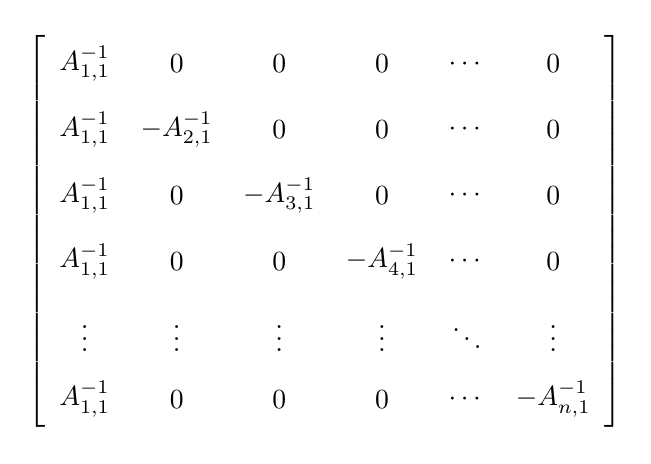
\begin{tikzpicture}[baseline={([yshift=-0ex]current bounding box.center)}]
\matrix(m) [matrix of nodes, row sep=1ex, column sep=1ex, nodes in empty cells, nodes={shape=rectangle,minimum height=3ex, anchor=center},ampersand replacement=\&] {
$A_{1,1}^{-1}$ \& $0$            \& $0$ \& $0$ \& $\cdots$ \& $0$ \\
$A_{1,1}^{-1}$ \& $-A_{2,1}^{-1}$ \& $0$        \& $0$ \& $\cdots$ \& $0$ \\
$A_{1,1}^{-1}$ \& $0$            \& $-A_{3,1}^{-1}$ \& $0$ \& $\cdots$ \& $0$ \\
$A_{1,1}^{-1}$ \& $0$            \&  $0$ \& $-A_{4,1}^{-1}$ \& $\cdots$ \& $0$ \\
$\vdots$       \& $\vdots$       \& $\vdots$  \& $\vdots$ \& $\ddots$ \& $\vdots$ \\
$A_{1,1}^{-1}$ \& $0$ \& $0$ \& $0$ \& $\cdots$ \& $-A_{n,1}^{-1}$\\
};
\node[fit= (m-1-1.north west) (m-6-6.south east), left delimiter={[}, right delimiter={]},inner sep=0ex] {};
\end{tikzpicture}
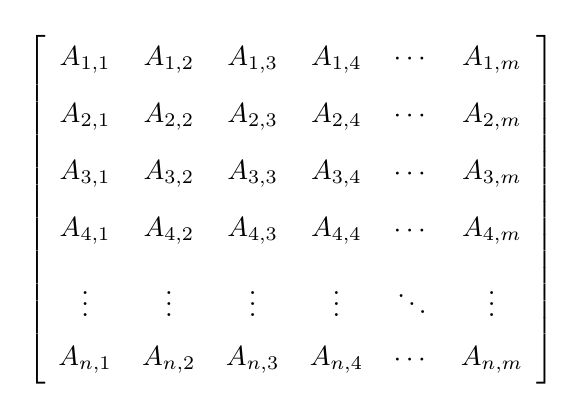
\begin{tikzpicture}[baseline={([yshift=-0ex]current bounding box.center)}]
\matrix(m) [matrix of nodes, row sep=1ex, column sep=1ex, nodes in empty cells, nodes={shape=rectangle,minimum height=3ex, anchor=center},ampersand replacement=\&] {
$A_{1,1}$ \& $A_{1,2}$ \& $A_{1,3}$ \& $A_{1,4}$ \& $\cdots$ \& $A_{1,m}$ \\
$A_{2,1}$ \& $A_{2,2}$ \& $A_{2,3}$ \& $A_{2,4}$ \& $\cdots$ \& $A_{2,m}$ \\
$A_{3,1}$ \& $A_{3,2}$ \& $A_{3,3}$ \& $A_{3,4}$ \& $\cdots$ \& $A_{3,m}$ \\
$A_{4,1}$ \& $A_{4,2}$ \& $A_{4,3}$ \& $A_{4,4}$ \& $\cdots$ \& $A_{4,m}$ \\
$\vdots$  \& $\vdots$ \& $\vdots$ \& $\vdots$ \& $\ddots$ \& $\vdots$ \\
$A_{n,1}$ \& $A_{n,2}$ \& $A_{n,3}$ \& $A_{n,4}$ \& $\cdots$ \& $A_{n,m}$\\
};
\node[fit= (m-1-1.north west) (m-6-6.south east), left delimiter={[}, right delimiter={]},inner sep=0ex] {};
\end{tikzpicture}    \\
& =
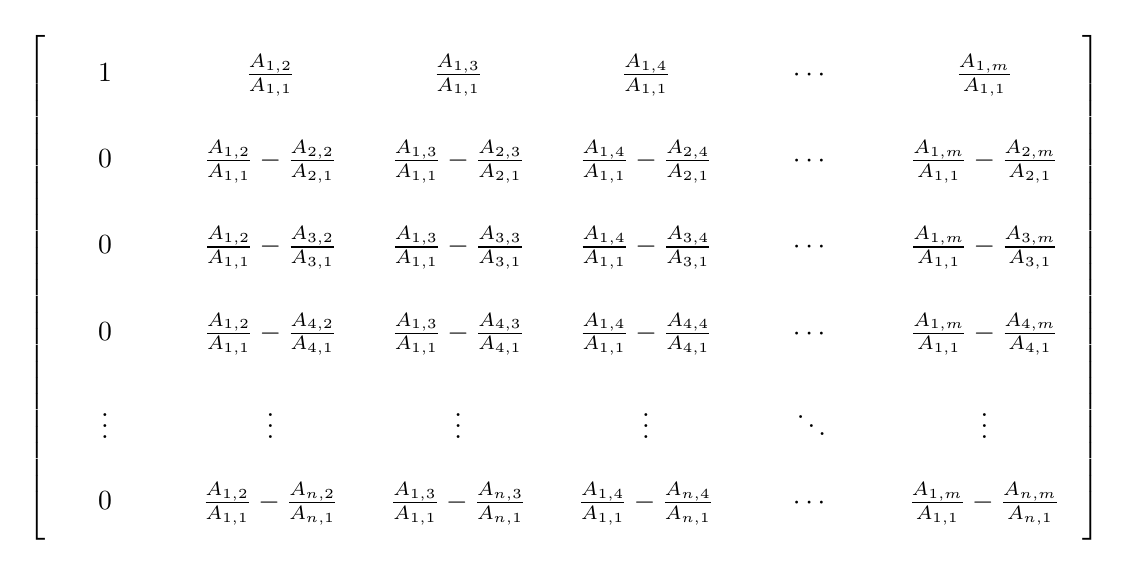
\begin{tikzpicture}[baseline={([yshift=-0ex]current bounding box.center)}]
\matrix(m) [matrix of nodes, row sep=1ex, column sep=2ex, nodes in empty cells, nodes={shape=rectangle,minimum height=6ex,
minimum width=10ex,align=center},ampersand replacement=\&] {
$1$ \& $\frac{A_{1,2}}{A_{1,1}}$ \& $\frac{A_{1,3}}{A_{1,1}}$ \& $\frac{A_{1,4}}{A_{1,1}}$ \& $\cdots$ \& $\frac{A_{1,m}}{A_{1,1}}$ \\
$0$ \& $\frac{A_{1,2}}{A_{1,1}}-\frac{A_{2,2}}{A_{2,1}}$ \& $\frac{A_{1,3}}{A_{1,1}}-\frac{A_{2,3}}{A_{2,1}}$ \& $\frac{A_{1,4}}{A_{1,1}}-\frac{A_{2,4}}{A_{2,1}}$ \& $\cdots$ \& $\frac{A_{1,m}}{A_{1,1}}-\frac{A_{2,m}}{A_{2,1}}$ \\
$0$ \& $\frac{A_{1,2}}{A_{1,1}}-\frac{A_{3,2}}{A_{3,1}}$ \& $\frac{A_{1,3}}{A_{1,1}}-\frac{A_{3,3}}{A_{3,1}}$ \& $\frac{A_{1,4}}{A_{1,1}}-\frac{A_{3,4}}{A_{3,1}}$ \& $\cdots$ \& $\frac{A_{1,m}}{A_{1,1}}-\frac{A_{3,m}}{A_{3,1}}$ \\
$0$ \& $\frac{A_{1,2}}{A_{1,1}}-\frac{A_{4,2}}{A_{4,1}}$ \& $\frac{A_{1,3}}{A_{1,1}}-\frac{A_{4,3}}{A_{4,1}}$ \& $\frac{A_{1,4}}{A_{1,1}}-\frac{A_{4,4}}{A_{4,1}}$ \& $\cdots$ \& $\frac{A_{1,m}}{A_{1,1}}-\frac{A_{4,m}}{A_{4,1}}$  \\
$\vdots$  \& $\vdots$ \& $\vdots$ \& $\vdots$ \& $\ddots$ \& $\vdots$ \\
$0$ \& $\frac{A_{1,2}}{A_{1,1}}-\frac{A_{n,2}}{A_{n,1}}$ \& $\frac{A_{1,3}}{A_{1,1}}-\frac{A_{n,3}}{A_{n,1}}$ \& $\frac{A_{1,4}}{A_{1,1}}-\frac{A_{n,4}}{A_{n,1}}$ \& $\cdots$ \& $\frac{A_{1,m}}{A_{1,1}}-\frac{A_{n,m}}{A_{n,1}}$  \\
};
\node[fit= (m-1-1.north west) (m-6-6.south east), left delimiter={[}, right delimiter={]},inner sep=0ex] {};
\end{tikzpicture}  
\end{align*}
$C$ is admissible as a basis transformation matrix only if $A_{i,1}\neq 0$ for all $i$.
Since,
\[
w_r=\sum_{j=1}^n C_{j,r} {\hat w}_j 
\]
and both $w_r$ and ${\hat w}_j$ are $n \times 1$ vectors, if $W$ is the matrix
whose columns are the $w$ basis vectors
and $\hat W$ is the matrix whose columns
are the $\hat w$ basis vectors then,
\[
W_{i,r} = \sum_{j=1}^n C_{j,r} {\hat W}_{i,j} 
\]
and therefore,
\[
W = {\hat W} C
\]
To express the new basis vectors in terms of the original basis we can right multiply both sides with $C^{-1}$ to get,
\[
{\hat W}=W C^{-1}
\]
It is easy to show that,
\[
C^{-1}=
\begin{tikzpicture}[baseline={([yshift=-3.5ex]current bounding box.center)}]
\matrix(m) [matrix of nodes, row sep=1ex, column sep=3ex, nodes in empty cells, nodes={shape=rectangle,minimum height=5ex, anchor=center},
            ampersand replacement=\&,] {
                \&  ${\hat w}_1$     \& ${\hat w}_2$  \& ${\hat w}_3$  \& ${\hat w}_4$  \& $\cdots$  \& ${\hat w}_n$ \\
    $w_1$       \& $A_{1,1}$         \& $0$           \& $0$           \& $0$           \&$\cdots$   \& $0$ \\
    $w_2$       \& $A_{2,1}$         \& $-A_{2,1}$    \& $0$           \& $0$           \&$\cdots$   \& $0$ \\
    $w_3$       \& $A_{3,1}$         \& $0$           \& $-A_{3,1}$    \& $0$           \&$\cdots$   \& $0$ \\
    $w_4$       \& $A_{4,1}$         \& $0$           \& $0$           \& $-A_{4,1}$    \&$\cdots$   \& $0$ \\
    $\vdots$    \& $\vdots$          \& $\vdots$      \& $\vdots$      \& $\vdots$      \& $\ddots$  \& $\vdots$\\
    $w_n$       \& $A_{n,1}$         \& $0$           \& $0$           \& $0$           \&$\cdots$   \& $-A_{n,1}$ \\
};
\node[fit= (m-2-2.north west) (m-7-7.south east), left delimiter={[}, right delimiter={]},inner sep=0ex] {};
\end{tikzpicture}
\]
and therefore,
\begin{align*}
    {\hat w}_1 &= \sum_{i=1}^n A_{i,1} w_i
    = T v_1 \\
    {\hat w}_i & = -A_{i,1} w_i \quad \text{ for }
    i>1
\end{align*}
\newline\noindent Why can't we go further and derive a basis of $W$ such that the first two entries in the first column of $\mathcal{M}(T)$ are equal to 1? Let's assume that a matrix $C$ exists with the property,
\begin{align*}
    \sum_{r=1}^n C_{1,r} A_{r,1} & =1 \\
    \sum_{r=1}^n C_{2,r} A_{r,1} & =1    
\end{align*}
This is only possible if $C_{1,r}=C_{2,r}$
i.e. if the first two rows of $C$ are identical. A matrix with two identical rows is not admissible as a basis transformation matrix. In order to prove this lets assume
that a matrix $C$ exists such that,
\[
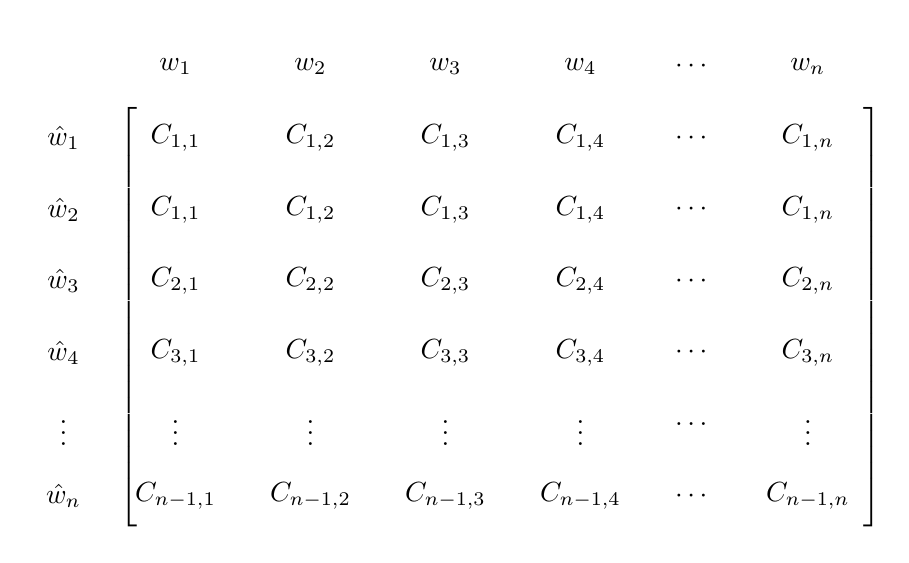
\begin{tikzpicture}[baseline={([yshift=-3.5ex]current bounding box.center)}]
\matrix(m) [matrix of nodes, row sep=1ex, column sep=3ex, nodes in empty cells, nodes={shape=rectangle,minimum height=5ex, anchor=center},
            ampersand replacement=\&,] {
                \&  ${w}_1$      \& ${w}_2$       \& ${w}_3$       \& ${w}_4$       \& $\cdots$  \& ${w}_n$ \\
 ${\hat w}_1$   \& $C_{1,1}$     \& $C_{1,2}$     \& $C_{1,3}$     \& $C_{1,4}$     \&$\cdots$   \& $C_{1,n}$ \\
 ${\hat w}_2$   \& $C_{1,1}$     \& $C_{1,2}$     \& $C_{1,3}$     \& $C_{1,4}$     \&$\cdots$   \& $C_{1,n}$  \\
 ${\hat w}_3$   \& $C_{2,1}$     \& $C_{2,2}$     \& $C_{2,3}$     \& $C_{2,4}$     \&$\cdots$   \& $C_{2,n}$ \\
  ${\hat w}_4$  \& $C_{3,1}$     \& $C_{3,2}$     \& $C_{3,3}$     \& $C_{3,4}$     \&$\cdots$   \& $C_{3,n}$ \\
 $\vdots$       \& $\vdots$      \& $\vdots$      \& $\vdots$      \& $\vdots$      \& $\dots$   \& $\vdots$\\
  ${\hat w}_n$  \& $C_{n-1,1}$   \& $C_{n-1,2}$   \& $C_{n-1,3}$   \& $C_{n-1,4}$ \&$\cdots$   \& $C_{n-1,n}$ \\
};
\node[fit= (m-2-2.north west) (m-7-7.south east), left delimiter={[}, right delimiter={]},inner sep=0ex] {};
\end{tikzpicture}
\]
Given that vectors ${\hat w}_i$ are independent we want to show that we can choose a set of constants $a_1,\ldots,a_n$
that are not all zero but for which,
\[
\sum_{i=1}^n a_i w_i=0
\]
Since,
\[
w_i = C_{1,i} \qty({\hat w}_1+{\hat w}_2)
+ \sum_{j=2}^n C_{j,i} {\hat w}_j
\]
we must have,
\[
\sum_{i=1}^n a_i 
\qty(C_{1,i} \qty({\hat w}_1+{\hat w}_2)
+ \sum_{j=2}^n C_{j,i} {\hat w}_j)
=0
\]
The last equation holds only if the coefficients of the ${\hat w}_j$ vectors are all zero, i.e,
\[
    \sum_{i=1}^n C_{j,i}a_i  = 0 
\]
for all $j$. Since $C$ is the matrix of a linear map
from a vector space with dimension $n$
to vector space with dimension $n-1$ this linear map cannot be injective; therefore the null set of this transformation contains non-zero vectors. 
It follows that $w_1,w_2,\ldots,w_n$ are not independent and a basis transformation matrix with two identical rows is not admissible.
}
\end{problem}
\newpage
\begin{problem}[3.D.2]
    { % problem
        Suppose $V$ is finite-dimensional and $\dim V>1$. Prove that the set of noninvertible operators on $V$
        is not a subspace of $\mathcal{L}(V)$.
    }
    { % solution
        If an operator $T$ is noninvertible it is also noninjective and nonsurjective since $V$ is finite-dimensional. 
        If an operator is nonsurjective then $\dim \range T < \dim V$ (this explains the condition $\dim V>1$ ; if $\dim V=1$
        then $\dim range T=0$, $T$ is an operator which maps all $v \in V$ to 0 and the set of operators with this property
        is a subspace). 
        
        We can choose two operators $T_1$ and $T_2$ with the following property: $\range T_1=\Span\{v_1,\ldots,v_r\}$
        and $\range T_2=\Span\{v_{r+1},\ldots,V_n\}$ where $n=\dim V$. Then $T_1+T_2$ has the property
        $\range T_1+T_2 = \Span\{v_1,\ldots,v_n\}=V$. Since $T_1+T_2$ is surjective it is also the case that it is invertible.
        Therefore the set of noninvertible operators is not closed under addition and is not a subspace of $\mathcal{L}(V)$.
     }
\end{problem}
\begin{problem}[3.D.3]
    {
        Suppose $V$ is finite-dimensional, $U$ is a subspace of $V$, and $S\in\lmap{U}{V}$.
        Prove there exists an invertible operator $T\in \mathcal{L}(V)$ such that $Tu=Su$
        for every $u\in U$ if and only if $S$ is injective.
    }
    {
        Since $U$ is a subspace of $V$ we can construct an operator $T\in\mathcal{L}(V)$
        with the property $Tu=Su$ for every $u\in U$. It is clear that since $S$ is injective in $U$, $T$ has
        the same property. For $v \in V\setminus U$, we can use the identity operator so that $Tv=Iv=v$ which is also 
        injective. Therefore, $T$ is injective for all $v \in V$; since an injective operator in finite dimensional
        space is also invertible it follows that $T$ is invertible.
        
        Now start with the condition that $T$ is an invertible operator in $\mathcal{L}(V)$; this implies it is also 
        injective. Since $Tu=Su$ for every $u \in U$, $S$ must also be injective.  
    }
\end{problem}
\begin{problem}[3.D.4]
    {
        Suppose $W$ is finite dimensional and $T_1,T_2\in \lmap{V}{W}$. Prove that 
        $\nspace T_1=\nspace T_2$ if and only if there exists an invertible operator 
        $S\in\mathcal{L}(W)$ such that $T_1=ST_2$.
    }
    {
        Start with $\nspace T_1=\nspace T_2$; $T_1v\neq 0 \Leftrightarrow Tv_2\neq 0$;
        define an operator $S$ using a construction as in the following graph:
        \begin{center}
        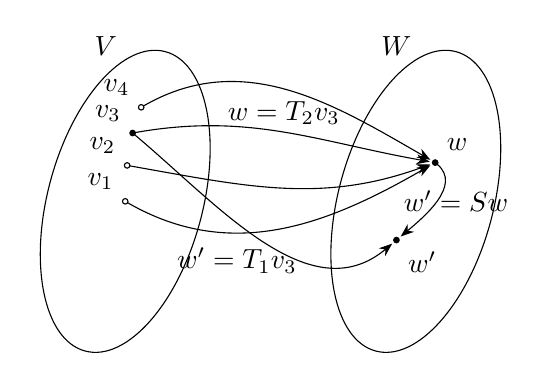
\begin{tikzpicture}[dot/.style = {circle, draw=black,fill=#1, minimum size=2pt,
            inner sep=0pt, outer sep=0pt},scale=.7]
            \draw[scale=2,rotate=-15,label=$V$] (0,0) ellipse (20pt and 40pt);
            \begin{scope}[xshift=150pt]
            \draw[scale=2,rotate=-15,label=$W$] (0,0) ellipse (20pt and 40pt);
            \node[dot,label=above right:$w$] (w) at (10pt,20pt) {};
            \node[dot,label=below right:$w'$] (w') at (-10pt,-20pt) {};
            \node at (-10pt,80pt) {$W$};
            \end{scope}
            \node at (-10pt,80pt) {$V$};
            %\draw (0,0) circle (1pt);
            \draw[draw=none] (0pt,0pt)arc [start angle=180, end angle=90, x radius=20pt, y radius=60pt]
            node [dot=none,pos=0,label=above left:$v_1$] (v1) {}
            node [dot=none,pos=0.2,label=above left:$v_2$] (v2) {}
            node [dot,pos=0.4,label=above left:$v_3$] (v3) {}
            node [dot=none,pos=0.6,label=above left:$v_4$] (v4){};
            \draw[-Stealth,shorten >=1pt] (v1) to[out=-30,in=210] (w);
            \draw[-Stealth,shorten >=1pt] (v2) to[out=-10,in=200] (w);
            \draw[-Stealth,shorten >=1pt] (v3) to[out=10,in=170] node[pos=0.5,yshift=7pt] {$w=T_2v_3$} (w) ;
            \draw[-Stealth,shorten >=1pt] (v4) to[out=30,in=150] (w);
            \draw[-Stealth,shorten >=1pt] (v3) to[out=-40,in=220] node[pos=0.5,yshift=-7pt,xshift=-10pt] {$w'=T_1v_3$} (w') ;
            \draw[-Stealth,shorten >=1pt] (w) to[out=-40,in=40] node[pos=0.5,xshift=7pt] {$w'=Sw$} (w') ;
        \end{tikzpicture}
        \end{center}
        For any $w \in \range T_2$ we can find a $v$ such that $w=T_2v$ (in the example above
        there are four different $v$s with this property so we choose $v_3$). For the same $v$,
        $w'=T_1v$ (it is possible that in some cases $w'=w$). The linear operator $S$ has the 
        property $w'=Sw$. Note that if $v \in \nspace T_2$, $T_2v=0$ and since $\nspace T_1=\nspace T_2$,
        $S0=0$ which is a property of any linear operator. From the definition of $S$, if $T_2v \neq 0$
        then $ST_2v=T_1v \neq 0$ and therefore $\nspace S=\{0\}$. This means $S$ is injective and using
        the properties of linear operators it is also invertible.
        
        Now assume that $S$ is an invertible linear operator with the property $T_1=ST_2$. For $v \in \nspace T_2$,
        $T_1v=ST_2v=S0=0$ and therefore $v \in \nspace T_1$. Since $S$ is invertible, $T_2=S^{-1}T_1$; 
        therefore for $v \in \nspace T_1$, $T_2v=S^{-1}T_1 v=S^{-1}0=0$ and $v \in \nspace T_2$. We conclude that
        $\nspace T_1=\nspace T_2$.
    }
\end{problem}

\tikzproblem[3.D.7]
    {
        Suppose $V$ and $W$ are finite-dimensional. Let $v\in V$. Let,
        $E=\{T \in \lmap{V}{W}:Tv=0\}$. Show that,
        \begin{enumerate}[a),itemsep=0pt,parsep=0pt]
            \item $E$ is a subspace of $\lmap{V}{W}$.
            \item Suppose $v\neq 0$. What is $\dim E$?
        \end{enumerate} 
    }
    {
        $E$ is a subspace of $\lmap{V}{W}$ if the following conditions hold:
        \begin{enumerate}[i),parsep=0pt,itemsep=0pt]
            \item Linear map $0 \in E$: since by definition $0v=0$ for all $v$
            this condition holds.
            \item $T_1,T_2 \in E \Rightarrow T_1+T_2 \in E$: since $T_1v=0$ and
            $T_2v=0$ we have $T_1v+T_2v=(T_1+T_2)v=0$.
            \item $T \in E,\; a \in \FF \Rightarrow aT \in E$: since $Tv=0$, 
            $aTv=0$ and therefore $aT \in E$.
        \end{enumerate}

        Any linear map $T \in \lmap{V}{W}$ can be represented by a matrix,
        \[
            \begin{tikzpicture}[baseline={([yshift=-0ex]current bounding box.center)}]
                \matrix(m) [matrix of nodes, row sep=1ex, column sep=3ex, nodes in empty cells, nodes={shape=rectangle,minimum height=5ex, anchor=center},
                            ampersand replacement=\&,] {
                                \&  $v_1$    \& $\cdots$ \& $v_j$     \& $\cdots$ \& $v_m$ \\
                 ${w}_1$   \& $A_{1,1}$ \& $\cdots$ \& $A_{1,j}$ \& $\cdots$ \& $A_{1,m}$ \\
                 $\vdots$       \& $\vdots$  \& $\ddots$ \& $\vdots$  \& $\ddots$ \& $\vdots$ \\
                 ${w}_i$   \& $A_{i,1}$ \& $\cdots$ \& $A_{i,j}$ \& $\cdots$ \& $A_{i,m}$ \\
                 $\vdots$       \& $\vdots$  \& $\ddots$ \& $\vdots$  \& $\ddots$ \& $\vdots$ \\
                 ${w}_n$   \& $A_{n,1}$ \& $\cdots$ \& $A_{n,j}$ \& $\cdots$ \& $A_{n,m}$ \\
                };
                \node[fit= (m-2-2.north west) (m-6-6.south east), left delimiter={[}, right delimiter={]},inner sep=0ex] {};
            \end{tikzpicture}
        \]
        whose elements are defined by,
        \[
        Tv_i = \sum_{j=1}^n A_{j,i} w_j    
        \]
        We can set the basis of $V$ to have $v_1=v$ without any loss of generality. Since $T\in E \Rightarrow Tv=0$
        a linear map $T\in E$ can be represented by the following matrix,
        \[
            \begin{tikzpicture}[baseline={([yshift=-2.5ex]current bounding box.center)}]
                \matrix(m) [matrix of nodes, row sep=1ex, column sep=3ex, nodes in empty cells, nodes={shape=rectangle,minimum height=3ex, anchor=center},
                            ampersand replacement=\&,] {
                           \&  $v_1$    \& $\cdots$ \& $v_j$     \& $\cdots$ \& $v_m$ \\
                 ${w}_1$   \& $0$ \& $\cdots$ \& $A_{1,j}$ \& $\cdots$ \& $A_{1,m}$ \\
                 $\vdots$  \& $\vdots$  \& $\ddots$ \& $\vdots$  \& $\ddots$ \& $\vdots$ \\
                 ${w}_i$   \& $0$ \& $\cdots$ \& $A_{i,j}$ \& $\cdots$ \& $A_{i,m}$ \\
                 $\vdots$  \& $\vdots$  \& $\ddots$ \& $\vdots$  \& $\ddots$ \& $\vdots$ \\
                 ${w}_n$   \& $0$ \& $\cdots$ \& $A_{n,j}$ \& $\cdots$ \& $A_{n,m}$ \\
                };
                \node[fit= (m-2-2.north west) (m-6-6.south east), left delimiter={[}, right delimiter={]},inner sep=0ex] {};
            \end{tikzpicture}
        \]
        The matrix representing $T\in\lmap{V}{W}$ is the linear combination of $n \times m$ basis 
        matrices each with zero for all elements except from $A_{i,j}=1$ i.e.,
        \[
        \mathcal{M}(T)=\sum_{i=1}^n \sum_{j=1}^m A_{i,j} \mathcal{M}_{i,j}   
        \]
        where,
        \[
            \mathcal{M}_{i,j} =
            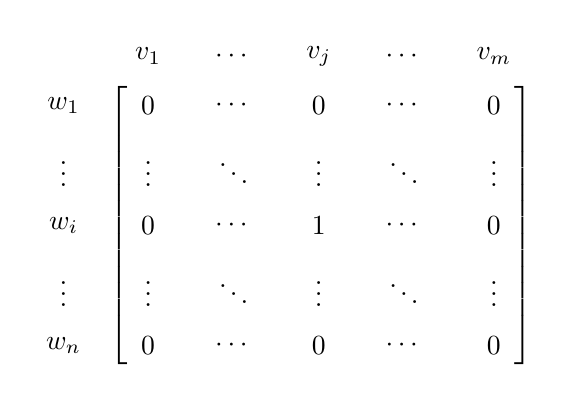
\begin{tikzpicture}[baseline={([yshift=-2.5ex]current bounding box.center)}]
                \matrix(m) [matrix of nodes, row sep=1ex, column sep=3ex, nodes in empty cells, nodes={shape=rectangle,minimum height=3ex, anchor=center},
                            ampersand replacement=\&,] {
                           \&  $v_1$    \& $\cdots$ \& $v_j$          \& $\cdots$ \& $v_m$ \\
                 ${w}_1$   \& $0$       \& $\cdots$ \& $0$    \& $\cdots$ \& $0$ \\
                 $\vdots$  \& $\vdots$  \& $\ddots$ \& $\vdots$     \& $\ddots$ \& $\vdots$ \\
                 ${w}_i$   \& $0$       \& $\cdots$ \& $1$          \& $\cdots$ \& $0$ \\
                 $\vdots$  \& $\vdots$  \& $\ddots$ \& $\vdots$     \& $\ddots$ \& $\vdots$ \\
                 ${w}_n$   \& $0$       \& $\cdots$ \& $0$          \& $\cdots$ \& $0$ \\
                };
                \node[fit= (m-2-2.north west) (m-6-6.south east), left delimiter={[}, right delimiter={]},inner sep=0ex] {};
            \end{tikzpicture}        
        \]
        For $T \in E$, $A_{i,1}=0$ for all $i$ and therefore,
        \[
            \mathcal{M}(T)=\sum_{i=1}^n \sum_{j=2}^m A_{i,j} \mathcal{M}_{i,j}   
        \] 
        i.e. the basis of $\mathcal{M}(T)$ consists of $(m-1)\times n$ matrices and therefore,
        \[
        \dim E = (m-1) n = (\dim V -1 ) \dim W    
        \]
    }

If $v \in V$ and $U$ is a subspace of $V$ the affine subset,
\[
v+U = \{v+u \, : \, u \in U \}    
\]
is said to be parallel  to $U$. Two affine subsets parallel to $U$ are either equal or disjoint.
To show that this is the case start with the assumption that $v+U \subset w+U$ and $w+U \not\subset v+U$.
Then there exists $u \in U$ s.t. $v+u \in w+U$; this means we can find $u' \in U$ s.t. $v+u=w+u'$. 
Rearanging terms we have $v-w+u=u'$; since $U$ is a subspace of $V$ this is only possible if $v-w \in U$
since $U$ is closed under addition. 

Next we want to show that there exists $u \in U$ s.t. $w+u \not\in v+U$. This means we cannot find any
$u' \in U$ s.t. $w+u = v+u'$; but this is not the case since $w+u=v+(w-v)+u$ and since $U$ is a subspace 
it is closed under scalar multiplication and addition, therefore, since $w-v, u \in U$, we have found
$u'=(w-v)+u$ so that $w+u = v+u'$. So $w+u \subset v+U$ and $v+U = w+U$.

For the disjoint case, start with $v+u \not\in w+U$; there is no $u' \in U$ s.t. $v+u=w+u'$. Lets assume
that $w+u \in v+U$, i.e. there is $u' \in U$ s.t. $w+u=v+u'$; since $U$ is a subspace, this means that
$w-v \in U$. If this is the case $v+u = w + (v-w)+u = w+u'$ and therefore $v+U \in w+U$ which contradicts our 
assumption. Therefore $v+U \cap w+U = \varnothing$.

\end{document}
